
\chapter{基于深度学习的骨髓血细胞检测算法设计与实现}
\section{引言}
骨髓血细胞形态学检查是血液疾病诊断的重要依据,主要通过人工镜检来完成,上述过程繁琐枯燥,可靠性差。
在骨髓血细胞自动化识别算法中,骨髓血细胞检测是将血细胞从涂片图像中定位并裁剪得到单一的血细胞图像,该过程是后续分类识别基础,
直接影响血液疾病诊断的结果,因此一直都是医学图像处理的热点研究方向之一。
目前基于深度学习的目标检测算法在很多领域都有广泛应用,如自动驾驶、安防监控、人脸识别、医学影像诊断等,其目的是定位或者跟踪相关目标。
本章提出了一种基于深度学习的改进RetinaNet骨髓血细胞自动化检测算法。

根据文献调研,目前血细胞检测主要是对血细胞图像中的红细胞、白细胞与血小板进行检测。
检测算法主要基于通用的深度学习目标检测算法,包括了单阶段检测算法与两阶段检测算法。
在两阶段方法中,通过区域举荐网络生成少量感兴趣区域,并将这些区域提取到的特征输入到后续的分类与回归分支中。
在单阶段算法中,如SSD、YOLO等网络直接将全部图像作为输入,学习类别概率与边界框位置。
两类方法各有优劣,本章第二节对这些方法进行阐述,并进行性能分析,最终选取性能较好的RetinaNet作为基线模型。

骨髓血细胞检测主要有如下三个难点:(1)相比外周血红细胞、白细胞、血小板三类血细胞检测,骨髓血细胞种类繁多、
形态丰富,尺寸大小不一。(2)在骨髓涂片制作过程中,由于染色剂与光照条件的变化,多个批次的数据存在着色彩差异。此外图像
背景复杂,存在较多成熟红细胞的干扰。(3)对于骨髓细胞增生活跃的切片,存在大量血细胞密集堆叠,边缘黏连,易导致漏检、错检等问题。
因此精准检测到骨髓血细胞是一项十分具有挑战性的课题。

针对上述难点,本章在第三节提出了一种改进RetinaNet网络,该方法提出了一种底向上的路径聚合网络结构,
缩短了底层与顶层特征之间的信息传递路径,提升了网络定位特征的提取能力。此外探究了不同标签分配策略对检测性能的影响,
基于最优输运的标签策略可以提高密集区域的血细胞检测精度。此外我们比较了空洞卷积、深度可分离卷积、可变形卷积等卷积网络,以期实现速度与检测精度的更优均衡。
在骨髓血细胞数据集上的实验结果表明,本文提出的改进方法在检测准确率上有较大的提升,达到了较为先进的性能。

\section{基于深度学习的骨髓血细胞检测网络}

\subsection{快速区域卷积神经网络}
快速区域卷积网络(Faster-RCNN)是目标检测领域最为经典的两阶段检测器,其网络架构如图\ref{fig:faster_rcnn}所示,主要由
骨干网络特征提取器(BackBone)、区域举荐网络(Region proposal Network,RPN)与分类回归网络(R-CNN)这三部分组成。骨干网络为深度卷积神经网络,
用于图像特征提取。RPN网络在提取的特征图上快速生成区域坐标与相应前景分数,这些区域用于后续的分类与坐标回归。
R-CNN网络对于这些区域首先进行ROI池化(Region of Interest Pooling)将区域转换为特定大小的特征图,然后这些特征图会分别进入到
分类分支与回归分支,得到待检测目标的类别与位置信息。

\begin{figure}  
   \centering   
   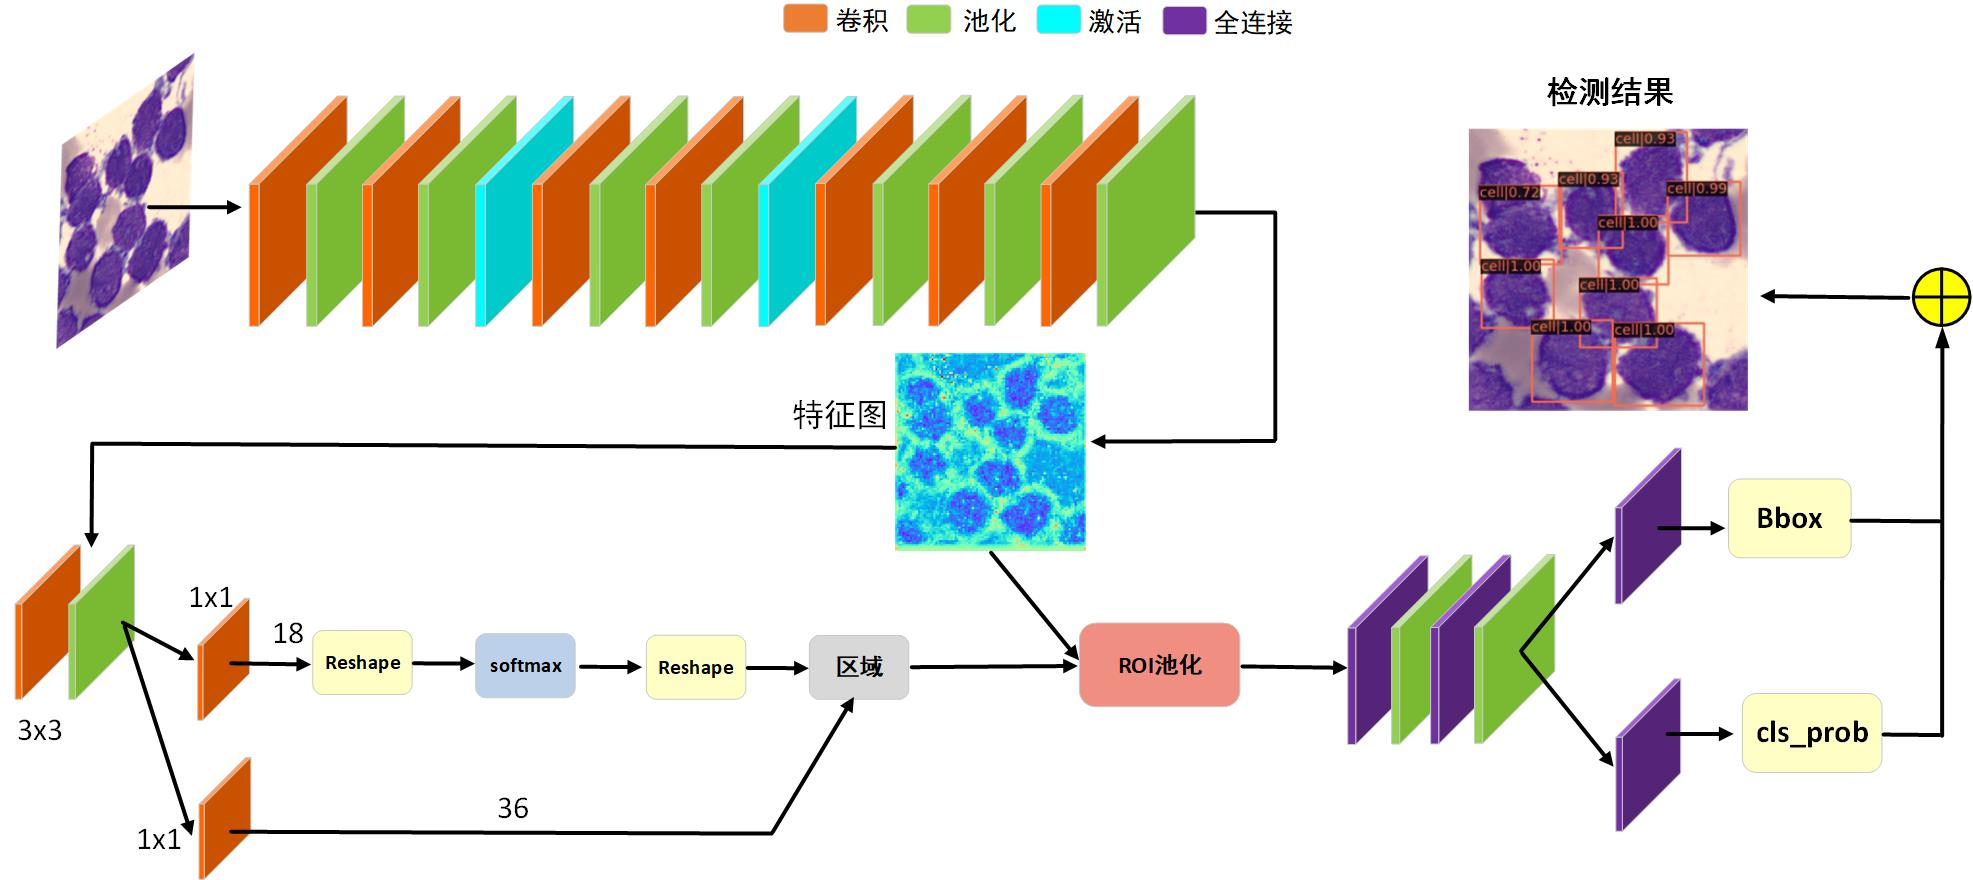
\includegraphics[width=1.0\linewidth]{faster_rcnn.jpg}   
   \caption{快速区域卷积神经网络结构示意图}   
   \label{fig:faster_rcnn} 
\end{figure}  

\subsubsection{骨干网络}
骨干网络是神经网络的主体部分,用于提取图像抽象的语义特征,为后续任务提供图像特征的嵌入向量表示。
因此,骨干网络的性能对于整体网络性能具有很大的影响。常用的骨干网络有VGG、ResNet、DenseNet与Inception等,
其中ResNet是应用最为广泛的骨干网络,其特点是引入了残差模块,可以实现非常深层的卷积网络。

综合考虑模型的精度、速度、参数量等因素,本节模型选择的骨干网络为ResNet50,其结构如图~\ref{}所示。
ResNet50总共由五个阶段(stage)构成,第一个阶段由一个$7\times7$的卷积与$3\times3$最大池化组成,可视作对图像的预处理。
其余阶段均是由结构类似的瓶颈结构(BottleNeck)堆叠而成,第二到第五阶段分别有3、4、6、3个瓶颈结构



\subsubsection{特征金字塔网络}
\subsubsection{RPN网络}
\subsubsection{分类与回归网络}

\subsection{单阶段RetinaNet检测网络}
\subsection{通用目标检测网络性能对比}

\section{改进的RetinaNet骨髓血细胞检测网络}
\subsection{路径聚合网络}
\subsection{基于最优输运的标签分配策略}
\subsection{卷积模块}
\section{算法实现与实验结果分析}
\subsection{实验环境}

\textbf{1)数据集介绍}

骨髓血细胞图像来自邃蓝智能科技(上海)有限公司合作医院提供,首先采用第2.1小节阐述的主动学习标注策略进行边界框的标注。
我们总共标记了6821张血细胞图像,训练集与测试集按照4:1的比例进行随机划分,训练集包含了5456张图像,测试集包含了1365张图像。
通常每个图像中包含1到10个有核血细胞,数据集总共标记了11352个血细胞,训练集有9065个血细胞,测试集有2287个血细胞。数据集的分布如
表~\ref{table:cell_detect}所示:

\begin{table}
  \caption{骨髓血细胞检测数据集分布}   
  \centering 
  \label{table:cell_detect}
  \begin{tabular}{ccccc}
    \toprule[2pt]
    序号 & 类别名  &  类别简写 & 训练集数量 & 测试集数量 \\
    \midrule[1.5pt] 
    1 & 原始细胞 & Prim & 1856 & 467 \\ 
    2 & 淋巴细胞 & Lym & 996 & 226   \\ 
    3 & 单核细胞 & Mono & 206 & 52   \\ 
    4 & 浆细胞 & Plas & 272 & 70   \\ 
    5 & 红细胞 & Red & 1880 & 503   \\ 
    6 & 早幼粒细胞 & Promy & 357 & 107   \\ 
    7 & 嗜中性中幼粒细胞 & Myelo & 701 & 150   \\ 
    8 & 嗜中性晚幼粒细胞 & Late & 503 & 144   \\ 
    9 & 嗜中性杆状核细胞 & Rods & 998 & 241   \\  
    10 & 嗜中分叶核细胞 & Lobu & 821 & 195   \\  
    11 & 嗜酸性粒细胞 & Eosl & 475 & 132   \\  
    \hline
    总计 &   &   & 9065 & 2287 \\
    \bottomrule[2pt]      
  \end{tabular} 
\end{table}
\subsection{消融实验}
\subsection{实验结果与分析}
\section{小结}


